% !TEX program = xelatex

\documentclass{beamer}

\usepackage[utf8]{inputenc}
\usepackage{ctex}

\usepackage{graphicx}
\usepackage{subcaption}

\usepackage{amsmath}
\usepackage{algorithm}
\usepackage{algpseudocode}



\graphicspath{ {images/} }

%\usetheme{albatross}
\usetheme{Madrid}
\usecolortheme{beaver}
%\usetheme{Antibes}


\title{Sprite sheet的生成 }
\author{卓越羿}
\institute[NUST]{}
\date{2018}

\begin{document}

\frame{\titlepage}

\begin{frame}

\frametitle{SpriteSheet}

Sprite 是一种游戏或图形应用中2d动画逻辑对象,SpriteSheet则是它的图像素材,
如图 \ref{fig:highpriest} 所示是RPGMaker的一个spritesheet的一部分,表示了
人物的四个方向的行走动作,共3帧。这种像素图在如图所示的小规模时尚易于绘制,
但精细的要求往往使得一个动作就有十几帧高分辨率图像,使得2d的sprite的制作
成本甚至还高于3d,这导致了所谓的3d渲染成2d的技术,不过这种技术对于一些并不
那么符合透视原理的设计并不适合。

\begin{figure}[htb]
    \centering
    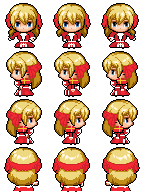
\includegraphics[width=0.3\linewidth]{H.png}
    \caption{Spritesheet例子}
    \label{fig:highpriest}
\end{figure}

\end{frame}

\end{document}